\documentclass[10pt]{article}

\usepackage[letterpaper,margin=1in]{geometry}
\usepackage[T1]{fontenc}
\usepackage{hyperref}
\usepackage[parfill]{parskip}
\usepackage{amsmath,amsfonts,amssymb,amsthm}
\usepackage{graphicx}
\usepackage{xcolor}

\graphicspath{{./figs/}}


\vspace{-8ex}
\date{}
\begin{document}

\title{\vspace{-1cm}\textbf{\Large{Intuitive Arm Reach}} \\ \Large{Project Formulation} \\ \textbf{\small{ECE496, 2021-22}}\\\vspace{-0.3cm}}
\author{Defne Dilbaz, Pranshu Malik, Prithvi Marwah, Varun Sampat \\\small{\textbf{Supervisor:}} Professor Mireille Broucke \vspace{-3cm}}

\maketitle

\section{Introduction}
To harness the complexity of their high-dimensional bodies during sensorimotor development, infants are guided by patterns of freezing and freeing of degrees of freedom. For instance, when learning to reach, infants free the degrees of freedom in their arm proximodistally, that is, from joints that are closer to the body to those that are more distant. that such patterns can emerge spontaneously as the result of a family of stochastic optimization processes, without an innate encoding of a maturational schedule. proximodistal organization appears spontaneously, which we denote PDFF (Proximo Distal Freezing and Freeing of degrees of freedom).
The Developmental Science article has a different focus, i.e. on modelling how infants learn to reach towards a certain position from scratch. The resulting differences to the robotics approach are: see appendix \ref{subsec:appendix_terms_def} for more information and terms.

Policy Since the aim is learning how to reach to a certain position, the policy should not have an attractor to that position (as in a DMP), because then there's nothing to learn anymore. Therefore, the policy is not a dynamical system with an attractor, but "just" a radial basis function network (equation 4)
Output (State) The policy generates accelerations in joint space (see equation 3). The underlying assumption is that infants have not yet learned inverse kinematics yet.
Initialization There is no initial trajectory. As mentioned in the article, The initial parameter vector is $\theta_\text{init}$ = 0, which means the arm is completely stretched, and not moving at all over time. Thus, the algorithm starts "from scratch" (as an infant), rather than from a demonstration.
Essentially, the assumptions one makes for robotics (attractor state as a goal, end-effector space generalizes better, warm start is good for optimization) are dropped in the Developmental Science work, because here we want to reduce the number of required auxillary hypotheses as much as possible to explain the observed data (the proximo-distal freezing/freeing over time). The goal of this project is to: <>.

\begin{figure}[h]
\centering
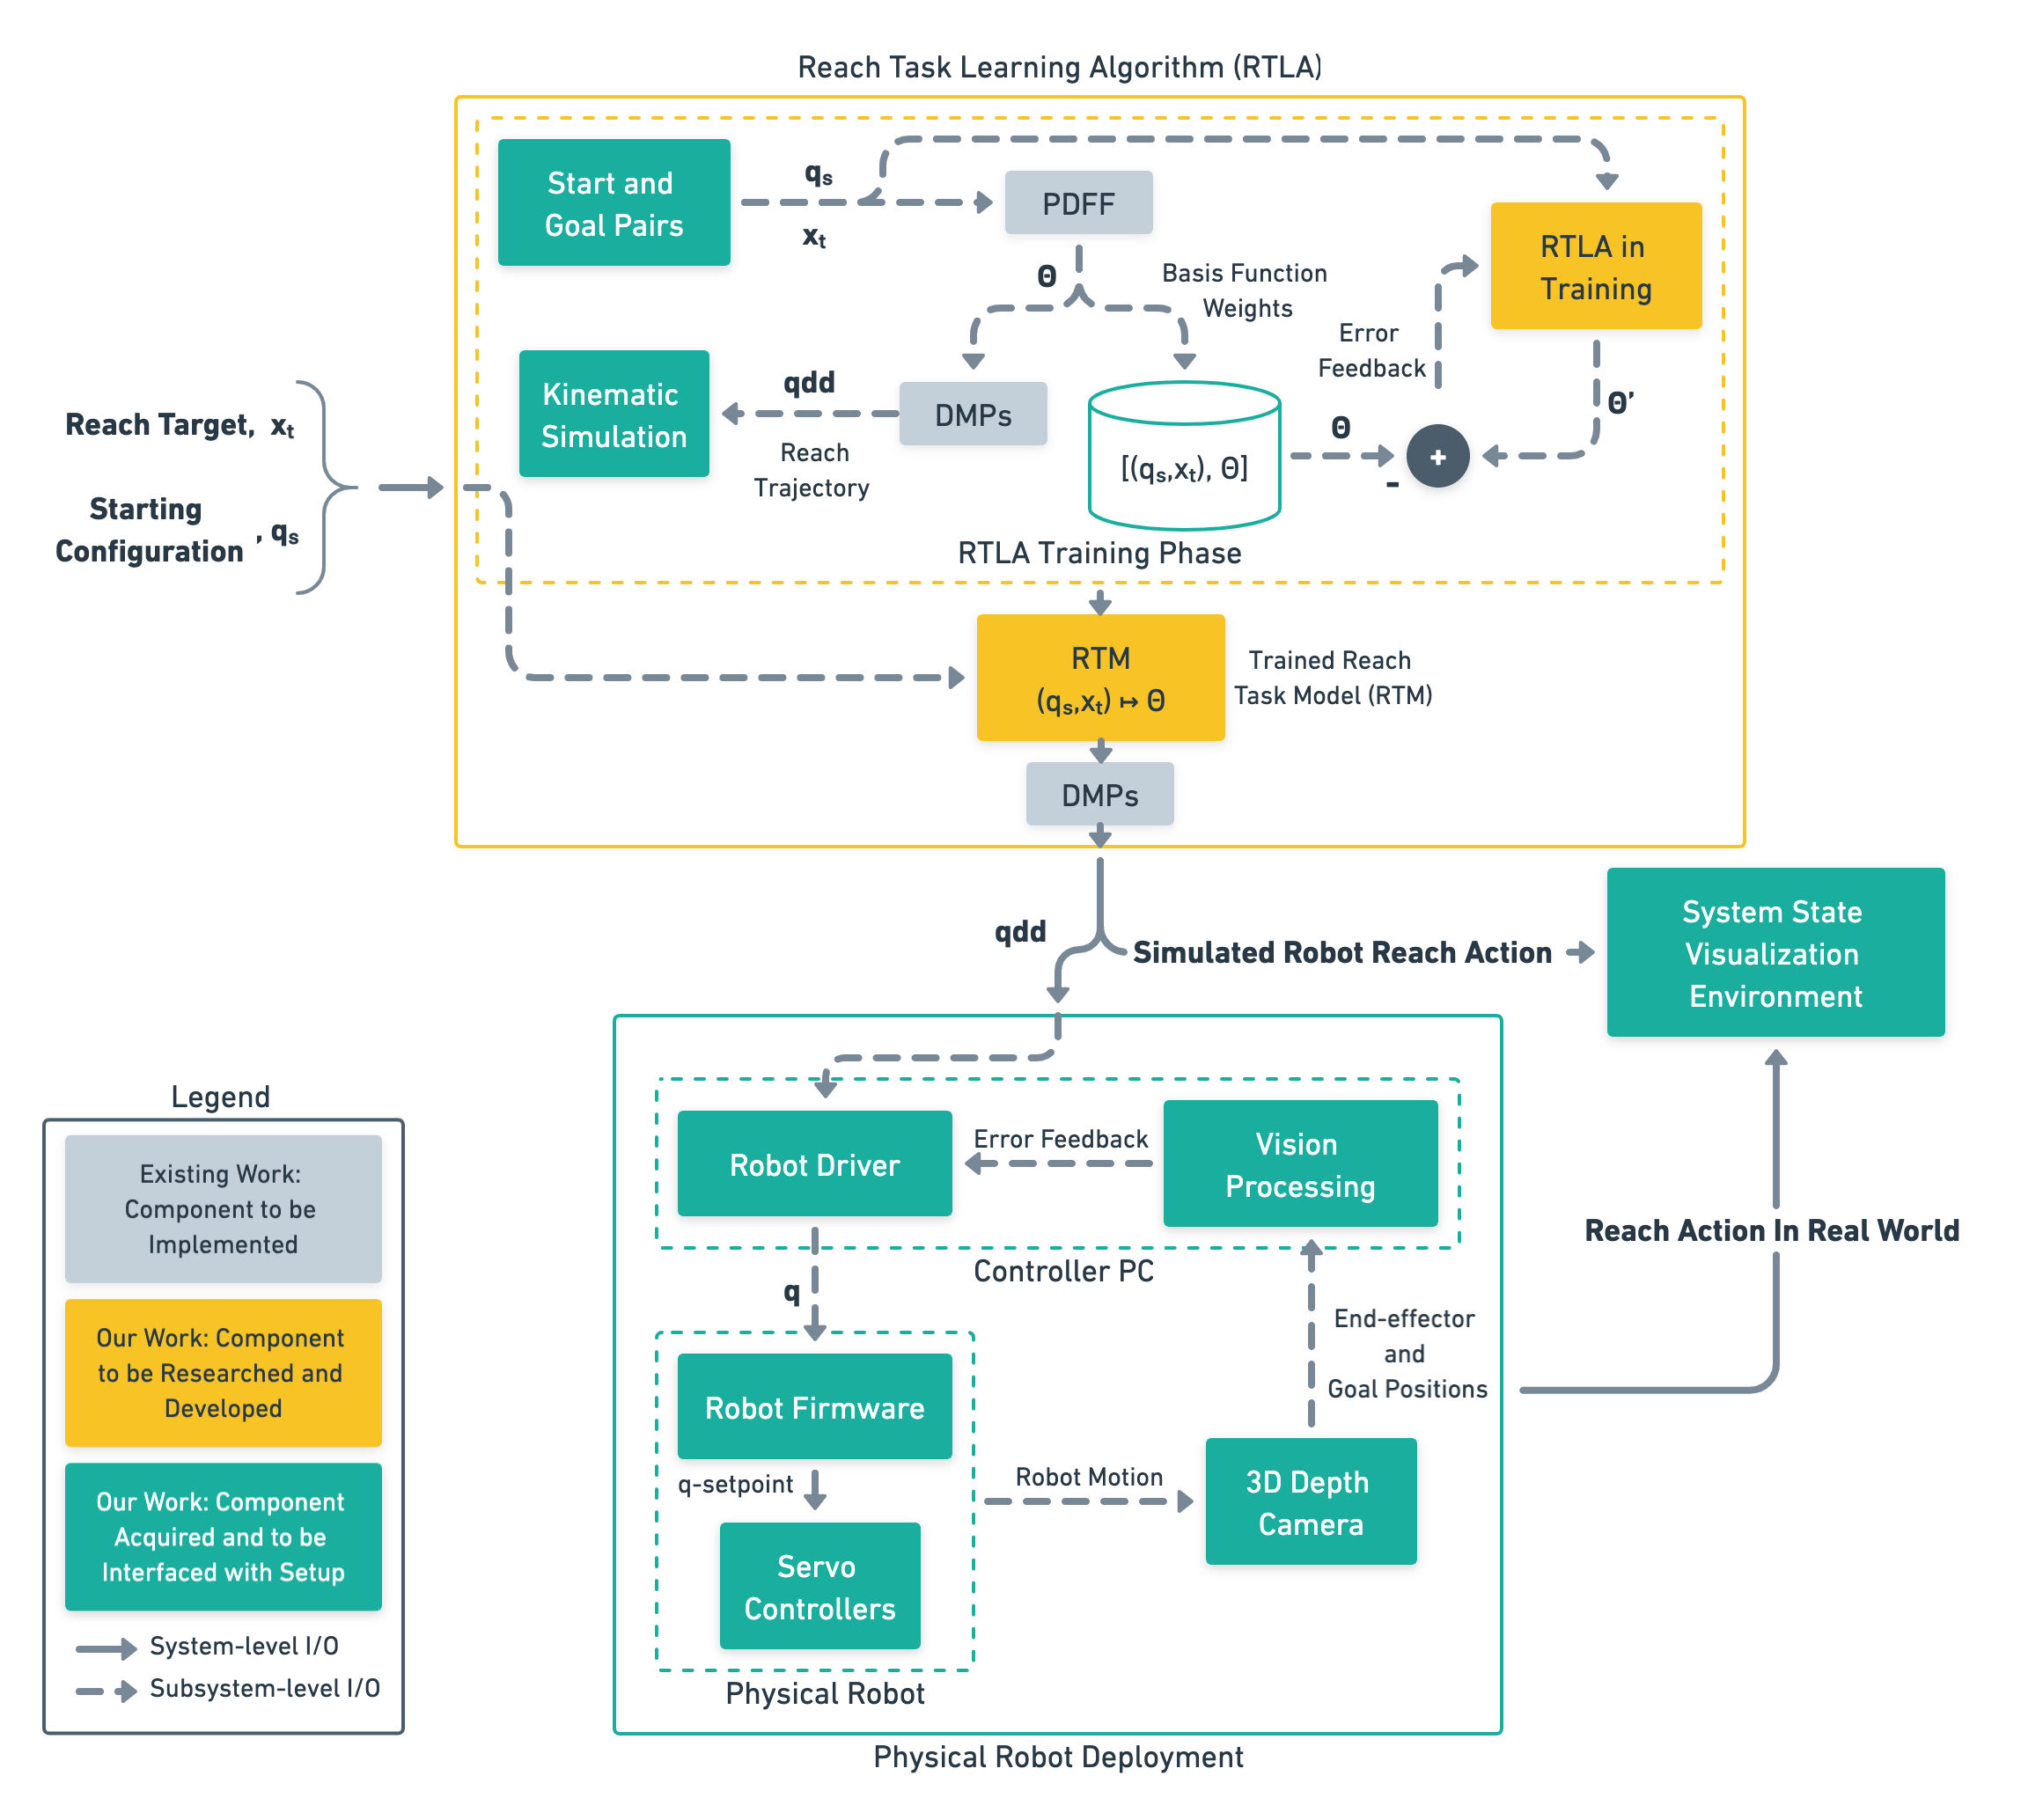
\includegraphics[width=0.7\textwidth]{system_level_overview.png}
\label{fig:system_level_overview}
\caption{System level overview}
\end{figure}

\section{Measurements and Knowns}
It should be clear what is known about the model and what are the measurements.

\section{Objective}

\section{Inputs}
$^{W}\xi_{E}$ and point of interest/reach $^{W}\xi_{O}$. $W$ is the inertial frame.

\section{Outputs}

\section{Training Algorithm}
\textcolor{red}{PDFF algo write}
Then prescribe what the function approximator RTM is going to do.

\subsection{Structure of training algorithm}

\section{Assumptions}

\section{Validation Procedure}

\begin{thebibliography}{5}
\bibitem{pdff}
 Stulp, Freek, and Pierre Yves Oudeyer. 2018. “Proximodistal Exploration in Motor Learning as an Emergent Property of Optimization.” Developmental Science 21 (4): 1–12. DOI: \href{https://doi.org/10.1111/desc.12638}{\texttt{10.1111/desc.12638}}.

\bibitem{dmps}
Jan Ijspeert, Auke, Jun Nakanishi, Heiko Hoffmann, Peter Pastor, and Stefan Schaal. n.d. “Dynamical Movement Primitives: Learning Attractor Models for Motor Behaviors.” Relevant  \href{http://www-clmc.usc.edu/Resources/Software}{\texttt{software}}.
\end{thebibliography}

\pagebreak

\appendix
\section*{Appendices}
\addcontentsline{toc}{section}{Appendices}
\renewcommand{\thesubsection}{\Alph{subsection}}
\subsection{Key Terms and Definitions}\label{subsec:appendix_terms_def}

\subsubsection{Arm Reach Problem}
Defined as <>

\subsubsection{Dynamical Movement Primitives (DMPs)}
This is a framework that helps in trajectory planning for dynamical systems to reach a target state. Dynamical Movement Primitives help modeling attractor behaviors of autonomous nonlinear dynamical systems with the help of statistical learning techniques. It models a simple dynamical system, defined by a set of linear differential equations, and then transforms them into a weakly nonlinear system with prescribed attractor dynamics by means of a learnable autonomous forcing term. Both point attractors and limit cycle attractors of almost arbitrary complexity can be generated.

\begin{equation}
    \ddot{y} = \alpha_y(\beta_y(y_g-y) - \dot{y}) + f
\end{equation}

Where $\alpha$ and $\beta$ are gain terms, $y$ is the system state, and $y_g$ is the goal state, and $f$ is the non-linear forcing function that helps achieve the goal and generate the trajectory. 

The forcing function $f$ is defined as:
\begin{equation}
    f(x,y_g) = \frac{\Sigma_{i = 1}^{N} \psi_i w_i}{\Sigma_{i = 1}^{N} \psi_i}  x(y_g - y)
\end{equation}
Where $w_i$ is the weighting given to its corresponding basis function $\psi_i$, and $x$ is defined as the canonical dynamical system with the dynamics: $\dot{x} = - \alpha_x x$.

The forcing function is set of Gaussians located 

Essentially, our forcing function is a set of Guassians that are activated as the canonical system $x$ converges to its target.  
 
\subsubsection{Human Motor Learning Processes}
Human motor learning processes define how humans develop motor skills. Examples of when these processes are used include how infants learn to reach objects or even when a teenager is attempting to learn a new sport. These processes develop internal models that humans use while performing a similar task. 
\textcolor{red}{Talk about human motor learning processes and DMP connection!!!}
\begin{itemize}
    \item PDFF: One such model is defined as the Proximodistal Exploration, which suggests that infants explore their surroundings by freezing and freeing (hence PDFF) their degrees of freedom. Mathematically, PDFF produces goal-directed movement by proximodistal exploration, i.e., by freezing and freeing of joints closest to the base to the furthest.
    
    The algorithm utilizes the math behind DMPs to generate accelarations in the joint space. Effectively, it has one DMP system for each joint of the arm, and it assumes that infants don't know how to reach objects already (inverse kinematics is not solved). 
    
    Here, the algorithm's objective to be able to reach all points in reachable space, and hence unlike DMPs there are no specific goals the system desires to reach => radial basis network
    
    Takes in arm model
    
    For each joint, PDFF models the joint acceleration using the math in DMPs:
    \begin{equation}
        \ddot{q}_{m,t} = \text{g}_t^\intercal\theta_m
    \end{equation}
    
    where $\theta_m$ is analogous to $w_m$ and $g_t$ is 
    
    
    
    \item Motor/Goal Babbling: Like PDFF, motor/goal babbling seeks inspiration from how human infants acquire their own body models as sensor-motor relationships. This can help a robot to learn by autonomously developing an internal model of its self-body and its environment, by making random movements and understanding its structure. The learning process includes how the system reaches a random set of points from a starting configuration. 
\end{itemize}

\end{document}